% !TeX program = lualatex
\documentclass[a0paper,landscape]{baposter}

\usepackage[EU1]{fontenc}
\usepackage{fontspec}
\defaultfontfeatures{Mapping=tex-text}
\setromanfont{TeX Gyre Schola}
\setsansfont{TeX Gyre Adventor}
\setmonofont{TeX Gyre Cursor}

\usepackage{setspace}

\usepackage[program=/home/jpv/lily2.20/bin/lilypond]{lyluatex}

\definecolor{lilyLightHeader1}{RGB}{212,242,201}
\definecolor{lilyLightHeader2}{RGB}{140,210,118}
\definecolor{lilyDarkHeader}{RGB}{91,127,100}


\begin{document}
\begin{poster}{%
	columns=5,
	background=none,
  % Show grid to help with alignment
	grid=false,
% Column spacing
	colspacing=1em,
% Color style
	bgColorOne=white,
	bgColorTwo=lilyLightHeader1,
	borderColor=lilyDarkHeader,
	headerColorOne=white,
	headerColorTwo=lilyLightHeader1,
	headerFontColor=lilyDarkHeader,
	boxColorOne=lilyLightHeader1,
	boxColorTwo=lilyLightHeader2,
% Format of textbox
	textborder=faded,
% Format of text header
	eyecatcher=true,
	headerborder=closed,
	headerheight=0.1\textheight,
%  textfont=\sc, An example of changing the text font
	headershape=rounded,
	headershade=shadetb,
%headerfont=\Large\bf\textsc, %Sans Serif
%textfont={\setlength{\parindent}{1.5em}},
	boxshade=plain,
%  background=shade-tb,
	background=plain,
	linewidth=2pt
	}
  {
  	
\includegraphics[width=0.14\linewidth]{double-lily-modified3.png}
  }
  {Lilypond}
  {Jan-Peter Voigt}
  {
\includegraphics[width=.14\textwidth]{double-lily-modified3.png}}
  
  \headerbox{Lilypond Usage}{name=lily1,column=0,span=2}{
  	
  }
  \headerbox{Johann Sebastian Bach}{name=marco,column=1,span=2,below=lily1}{
  	The St.Mark Passion by Johann Sebastian Bach
  }
  
  \headerbox{Contempory Music}{name=keller,column=3,span=2}{
	Excerpts from Hermann Keller's composition for speaking cellist\\
	"Ihr sollt die Wahrheit erben"
	
    %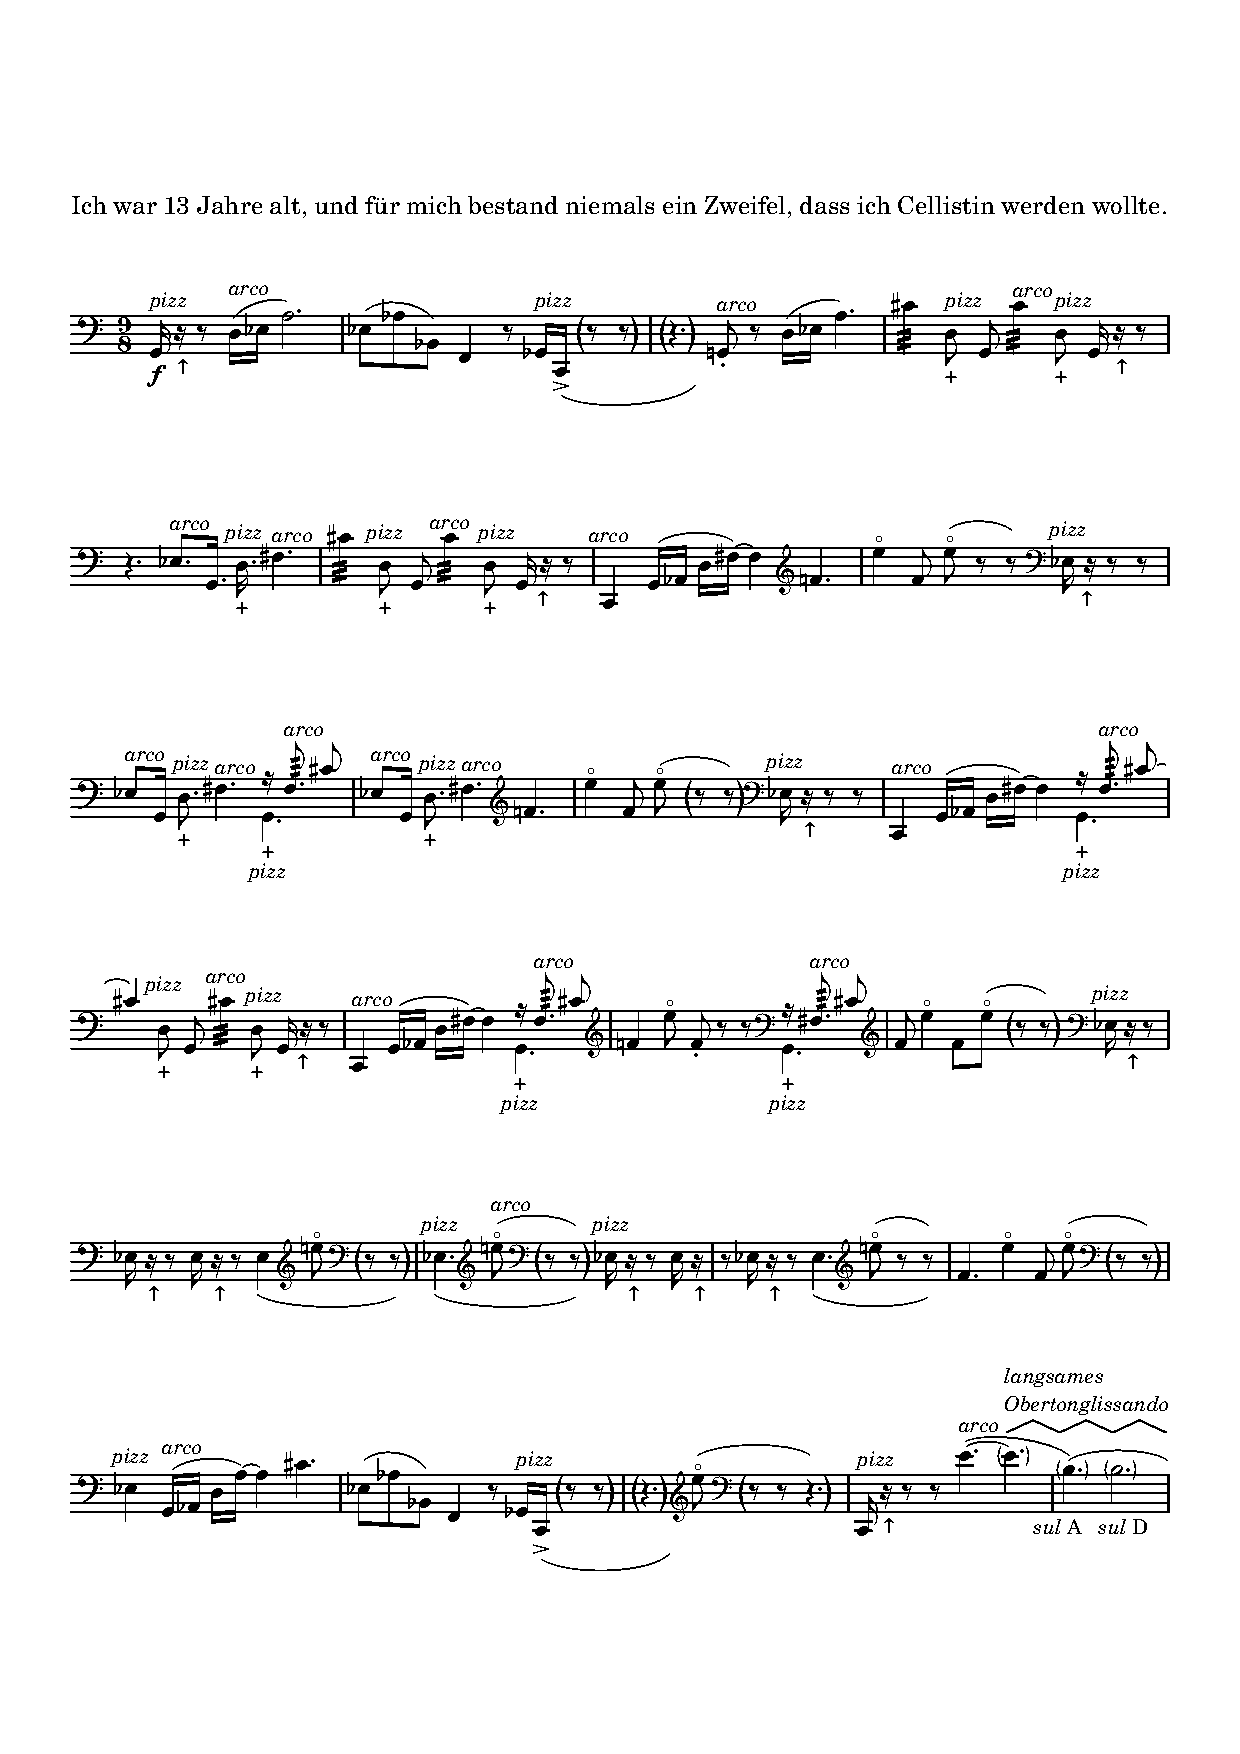
\includegraphics[width=.5\textwidth]{wahrheit1}
    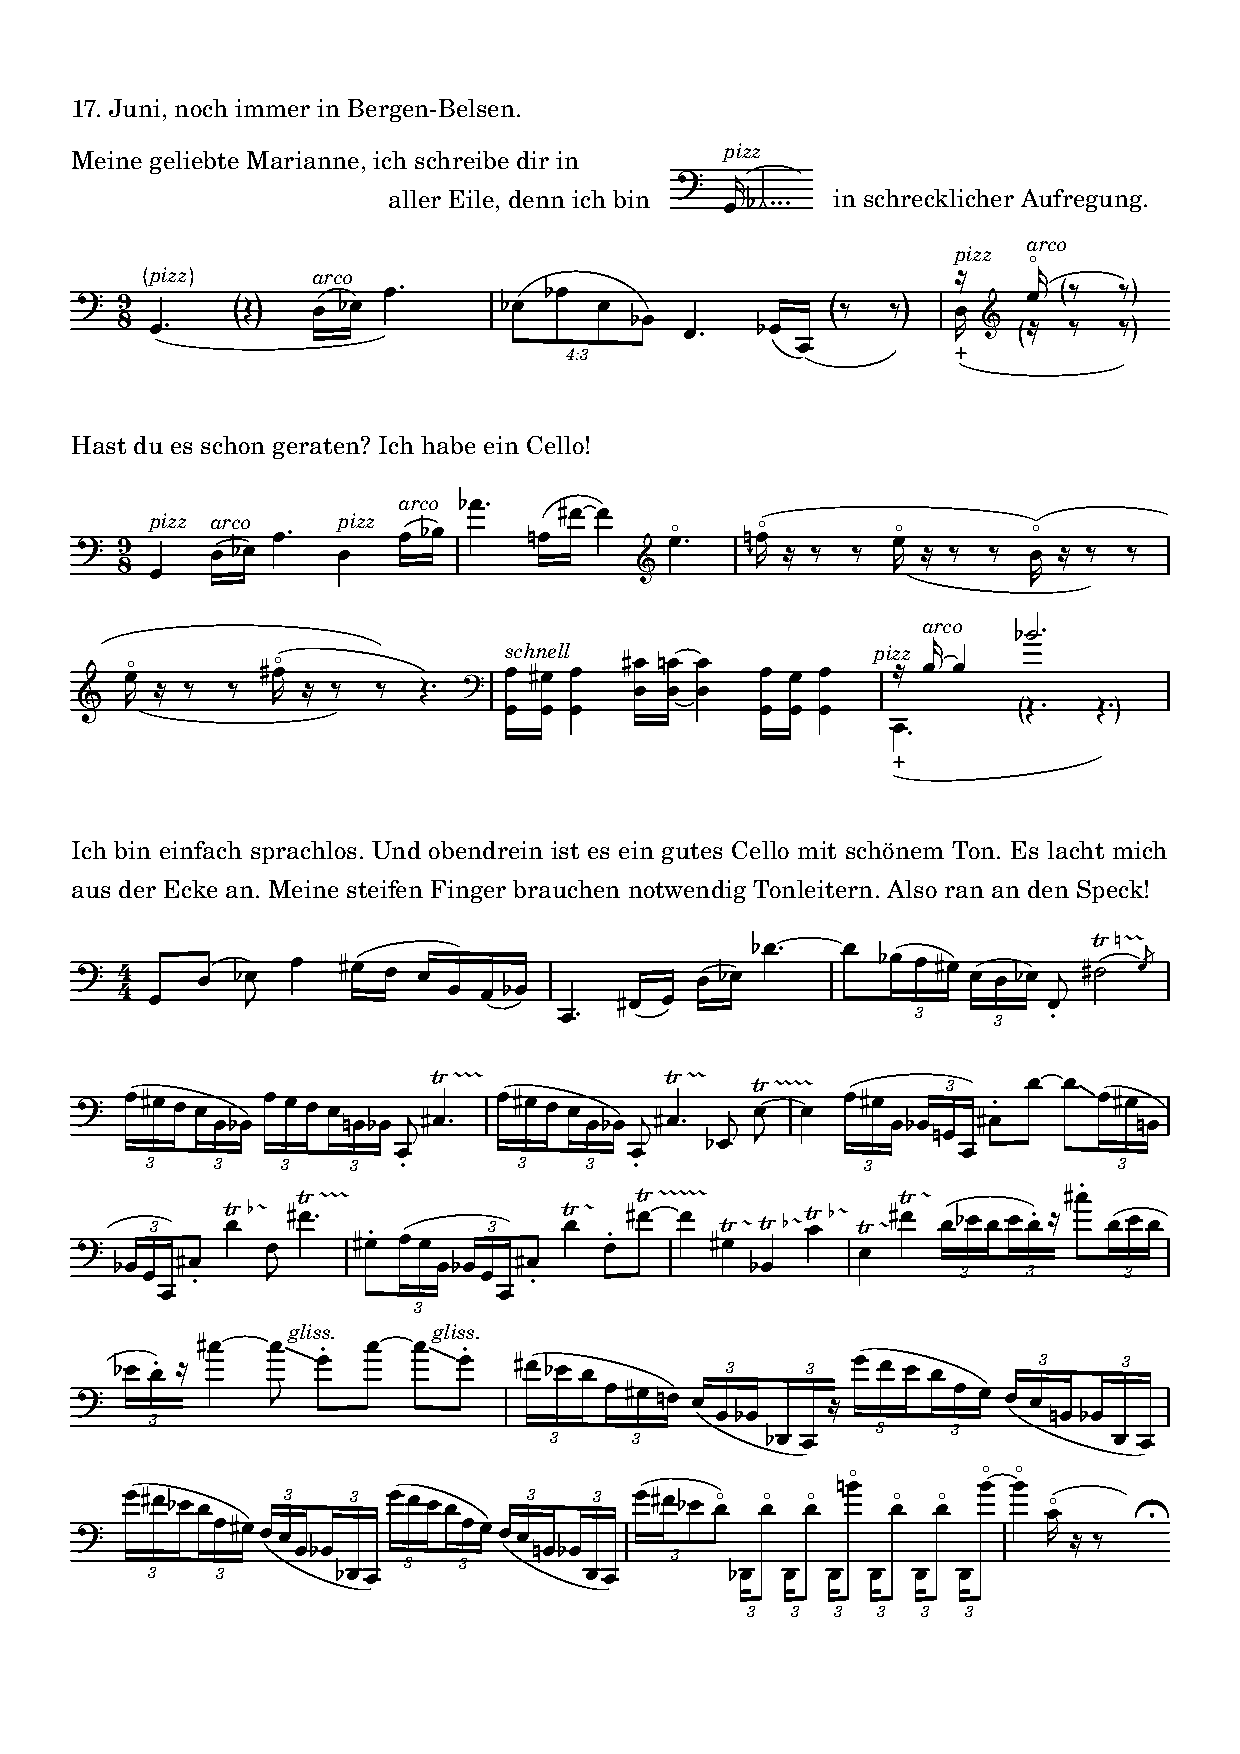
\includegraphics[width=\textwidth]{wahrheit2}
	    
	{\scriptsize © 2019 Edition Juliane Klein, Berlin $\bullet$
	\emph{The excerpts are reproduced with the kind permission of the publisher.}}
    }
\end{poster}
\end{document}
